\tikzset{>=latex} % for LaTeX arrow head
\colorlet{Ecol}{orange!90!black}
\tikzstyle{charge0}=[top color=green!80!black!50,bottom color=green!80!black,shading angle=20]
\tikzstyle{charge+}=[top color=red!50,bottom color=red!70!black,shading angle=20]
\tikzstyle{charge-}=[top color=blue!50,bottom color=blue!80,shading angle=20]
\tikzstyle{metal}=[top color=black!15,bottom color=black!25,middle color=black!5,shading angle=10]
\tikzset{
  EField/.style={thick,Ecol,decoration={markings,
                 mark=at position #1 with {\arrow{latex}}},
                 postaction={decorate}},
  EField/.default=0.5}

% CONDUCTION MODEL
\def\R{0.21} % ion radius
\def\a{0.90} % scale
\def\Rx{0.2*\a*\Ny}
\def\Ry{0.5*\a*\Ny}
\def\Nx{6} % number of ions columns
\def\Ny{3} % number of ions rows
\def\L{\a*(\Nx-1)} % length
\def\electron#1#2#3{
  \node[charge-,draw=black,circle,fill,inner sep=0.8,scale=0.5,line width=0.3]
    (e) at (#1*\a,#2*\a) {$\bm-$};
  \draw[->,green!60!black] (e) --++ (#3*0.7*\a);
}


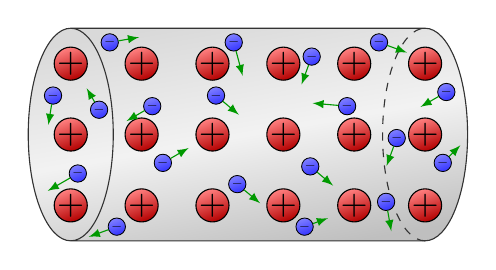
\begin{tikzpicture}
  
  \fill[metal] (0,{-\Ry}) arc (270:90:{\Rx} and {\Ry}) --++ ({\L},0) arc (90:-90:{\Rx} and {\Ry});
  \draw[black!80] (0,{-\Ry}) arc (270:90:{\Rx} and {\Ry});
  \draw[black!80,dashed] ({\L},{-\Ry}) arc (270:90:{\Rx} and {\Ry});
  
  % IONS
  \foreach \j [evaluate={\y=\a*(\j-\Ny/2-0.5);}] in {1,...,\Ny}{
    \foreach \i in {1,...,\Nx}{ %[evaluate={\x=\j*\a;}]
      \draw[charge+] ({(\i-1)*\a},\y) circle (\R) node[scale=1.4*\a,inner sep=1] {$+$};
    }
  }
  
  %%%%%%%%%%%%%%%%%%%%%%%%%%%%%%%%% 0
  \electron{-0.25}{ 0.55}{ -99:0.6}
  %%%%%%%%%%%%%%%%%%%%%%%%%%%%%%%%% 1
  \electron{ 0.10}{-0.55}{ 210:0.7}
  \electron{ 0.40}{ 0.35}{ 120:0.5}
  \electron{ 0.55}{ 1.30}{  10:0.6}
  %%%%%%%%%%%%%%%%%%%%%%%%%%%%%%%%% 2
  \electron{ 0.65}{-1.30}{-160:0.6}
  \electron{ 1.30}{-0.40}{  30:0.6}
  \electron{ 1.15}{ 0.40}{ 210:0.6}
  %%%%%%%%%%%%%%%%%%%%%%%%%%%%%%%%% 3
  \electron{ 2.35}{-0.70}{ -40:0.6}
  \electron{ 2.05}{ 0.55}{ -40:0.6}
  \electron{ 2.30}{ 1.30}{ -75:0.7}
  %%%%%%%%%%%%%%%%%%%%%%%%%%%%%%%%% 4
  \electron{ 3.30}{-1.30}{  20:0.5}
  \electron{ 3.40}{ 1.10}{-110:0.6}
  %%%%%%%%%%%%%%%%%%%%%%%%%%%%%%%%% 5
  \electron{ 3.38}{-0.45}{ -40:0.6}
  \electron{ 3.90}{ 0.40}{ 175:0.7}
  \electron{ 4.35}{ 1.30}{ -20:0.6}
  %%%%%%%%%%%%%%%%%%%%%%%%%%%%%%%%% 6
  \electron{ 4.45}{-0.95}{ -80:0.6}
  \electron{ 5.25}{-0.40}{  45:0.5}
  \electron{ 4.60}{-0.05}{-110:0.6}
  \electron{ 5.30}{ 0.60}{-150:0.6}
  %%%%%%%%%%%%%%%%%%%%%%%%%%%%%%%%%
  
  \draw[black!80] (0,{-\Ry}) arc (-90:90:{\Rx} and {\Ry}) --++ ({\L},0) arc (90:-90:{\Rx} and {\Ry}) -- cycle;
  
\end{tikzpicture}
